\documentclass{article}
\usepackage{listings}
\usepackage{graphicx}
\title{Operational Statistics for SAR Imagery Report}
\author{Chen Yang}
\date\today
\begin{document}
\maketitle
\section{sample Image}
\begin{lstlisting}[frame=tb]

> imagepath <- "../Data/Images/ESAR/"

> HH_Complex <- myread.ENVI(paste(imagepath,
 "ESAR97HH.DAT", sep = ""), 
paste(imagepath, "ESAR97HH.hdr", sep = ""))
> HH_Intensity <- (Mod(HH_Complex))^2
> example <- HH_Intensity[1500:1599,1500:1599]
> vexample <- data.frame(HH=as.vector(example))
> summary(vexample)
       HH          
 Min.   :       5  
 1st Qu.:   49397  
 Median :  139494  
 Mean   :  486161  
 3rd Qu.:  382280  
 Max.   :34400251 
> plot(imagematrix(equalize(example))) (figure.1)
\end{lstlisting}

\begin{figure}[htb]
	\centering
	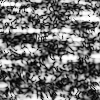
\includegraphics[width=0.5\linewidth]{example.png}
	\caption{}
	\label{fig:example}
\end{figure}



\section{Histogram}
\begin{lstlisting}[frame=tb]
> binwidth_complete <- 2*IQR(vexample$HH)*length(vexample$HH)^(-1/3)
> ggplot(data=vexample, aes(x=HH)) + 
+   geom_histogram(aes(y=..density..), 
+                  binwidth = binwidth_complete) + 
+   xlab("Intensities") +
+   ylab("Proportions") +
+   ggtitle("Complete Histogram") +
+   theme_few()
\end{lstlisting}
\begin{figure}
	\centering
	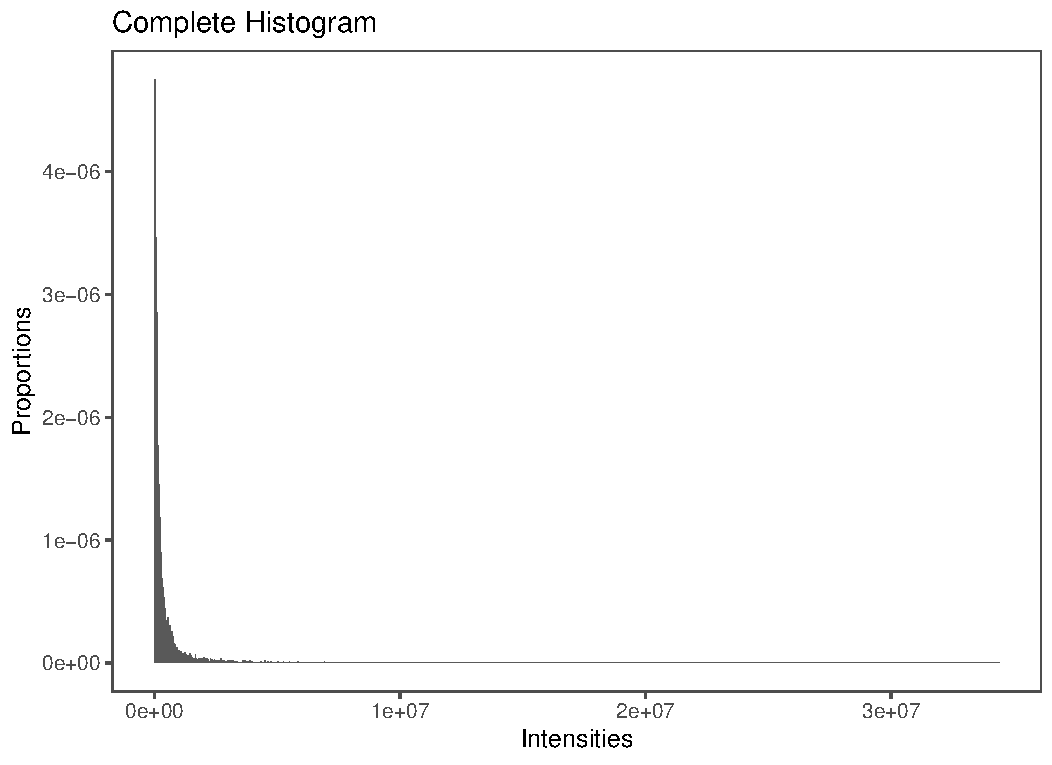
\includegraphics[width=0.5\linewidth]{HistogramExample.pdf}
	\caption{}
	\label{fig:HistogramExample}
\end{figure}

\section{LogLikelihood}
\begin{lstlisting}[frame=tb]
> LogLikelihoodLknown <- function(params) {
+   
+   p_alpha <- -abs(params[1])
+   p_gamma <- abs(params[2])
+   p_L <- abs(params[3])
+   n <- length(z)
+   return(
+     n*(lgamma(p_L-p_alpha) - p_alpha*log(p_gamma) - lgamma(-p_alpha)) + 
+       (p_alpha-p_L)*sum(log(p_gamma + z*p_L)) 
+   )
+ }
\end{lstlisting}
\section{Estimation}
\begin{lstlisting}[frame=tb]
> estim.exampleML <- maxNR(LogLikelihoodLknown, 
+                        start=c(estim.example$alpha, estim.example$gamma,1), 
+                        activePar=c(TRUE,TRUE,FALSE))$estimate[1:2]
> estim.exampleML
[1] -3.866783e+00  1.080319e+06
\end{lstlisting}
results all above
\end{document}
